\documentclass[a4paper,12pt]{article}

\usepackage[utf8]{inputenc}
\usepackage[T1]{fontenc}
\usepackage[english]{babel}
\usepackage{geometry}
\usepackage{graphicx}

\geometry{margin=1in}

\title{Quiz Game Description}
\author{}
\date{}

\begin{document}

\maketitle

\section{Introduction}
\subsection{How to compile project}
Ensure you have the following installed:
\begin{itemize}
    \item g++
    \item make
\end{itemize}

To compile the project, copy the content of one from the folders below into a \texttt{Makefile}
\begin{itemize}
    \item \texttt{compiled/makefiles/makefileWindows.makefile} - for windows
    \item \texttt{compiled/makefiles/makefileLinux.makefile} - for Linux
\end{itemize}
In root of the project in terminal run: make. \newline
Or another way to compile the project is to move script\
\texttt{compiled/makefiles/windowsCompile.bat}.

\section{Game Description}
base idea:
The quiz game will be about testing the user's knowledge in various categories.\
The game will present single-choice questions. Questions will be presented one\
at a time.

\section{Implementation}
There will bew used MVC pattern.\
\subsection{Model}
There will be all logic of the game.
\subsection{View}
Currently the view can be implemented in console.\
In future it can be in GUI.
\subsection{Controller}
The controller will be responsible for communication between\
the model and the view. It will also handle the user input and\
update the model accordingly.\newline \newline

\begin{figure}[h]
    \centering
    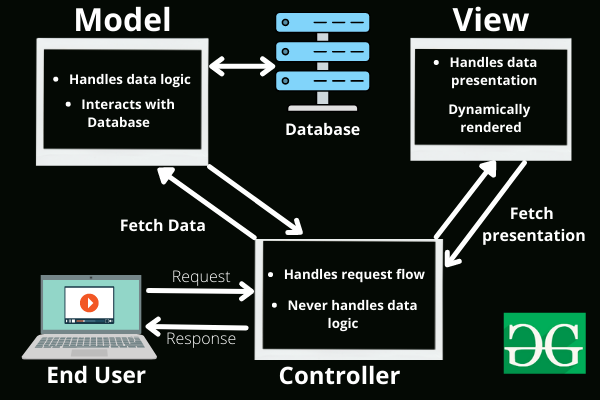
\includegraphics[width=0.5\textwidth]{images/Model1.png}
    \caption{The image represents the way like MVC should work.}
    \label{fig:class_diagram}
\end{figure}



\section{Technologies Used}
\begin{itemize}
    \item C++ - with STL libraries
    \item make - for building the project
    \item g++ - for compiling the project
    \item git - for version control
\end{itemize}

\section{Ideas for Future Development}
\begin{itemize}
    \item Add more question categories. - obviously, currently there are none
    \item Implement a scoring system. - maybe
    \item Create a user-friendly interface. - now is only needed simple or console
    \item Add a timer for each question. - maybe
    \item few categories of questions - knowledge or knowledge about another person
    \item Add multiplayer functionality. - category like in cozy app and category where like opponents
\end{itemize}
% \section{Features}
% \begin{itemize}
%     \item Multiple-choice questions.
%     \item Timed quizzes to challenge users.
%     \item Score tracking and leaderboard.
%     \item User-friendly interface.
% \end{itemize}

% \section{Game Flow}
% \begin{enumerate}
%     \item The user starts the game and selects a category.
%     \item A series of questions is presented, one at a time.
%     \item The user selects an answer within the given time limit.
%     \item The game calculates the score and displays the results.
% \end{enumerate}

% \section{Future Enhancements}
% \begin{itemize}
%     \item Add support for multiplayer mode.
%     \item Include more diverse question categories.
%     \item Implement hints and lifelines for difficult questions.
% \end{itemize}

\end{document}